\section{Softwarearchitektur}
\label{sec:Softwarearchitektur}

\begin{figure}[H]
  \centering
  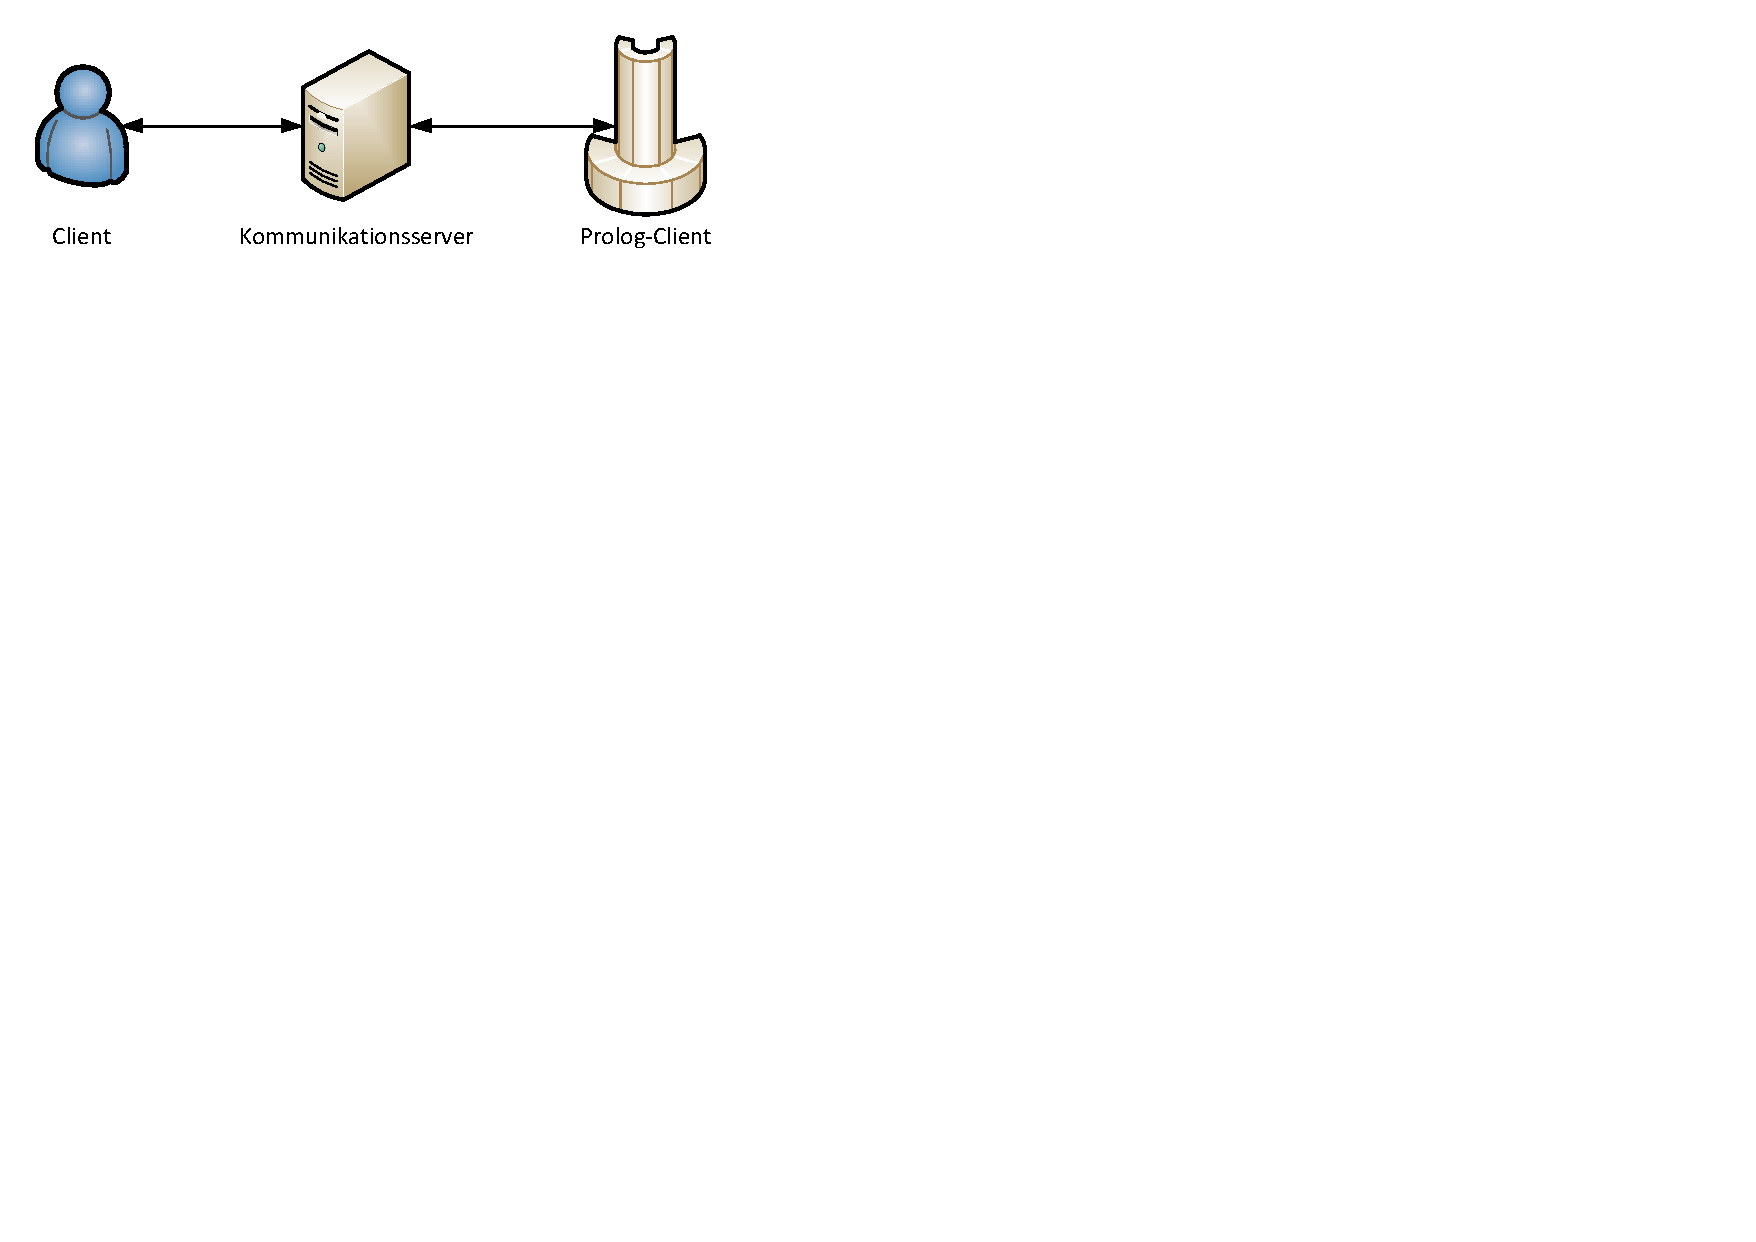
\includegraphics[trim=0mm 165mm 175mm 0mm,clip,width=0.5\textwidth]{images/Kommunikationsmodell.pdf}
  \caption{Darstellung der möglichen Kommunikationsteilnehmer}
  \label{fig:Kommunikationsteilnehmer}
\end{figure}


\begin{figure}[H]
  \centering
  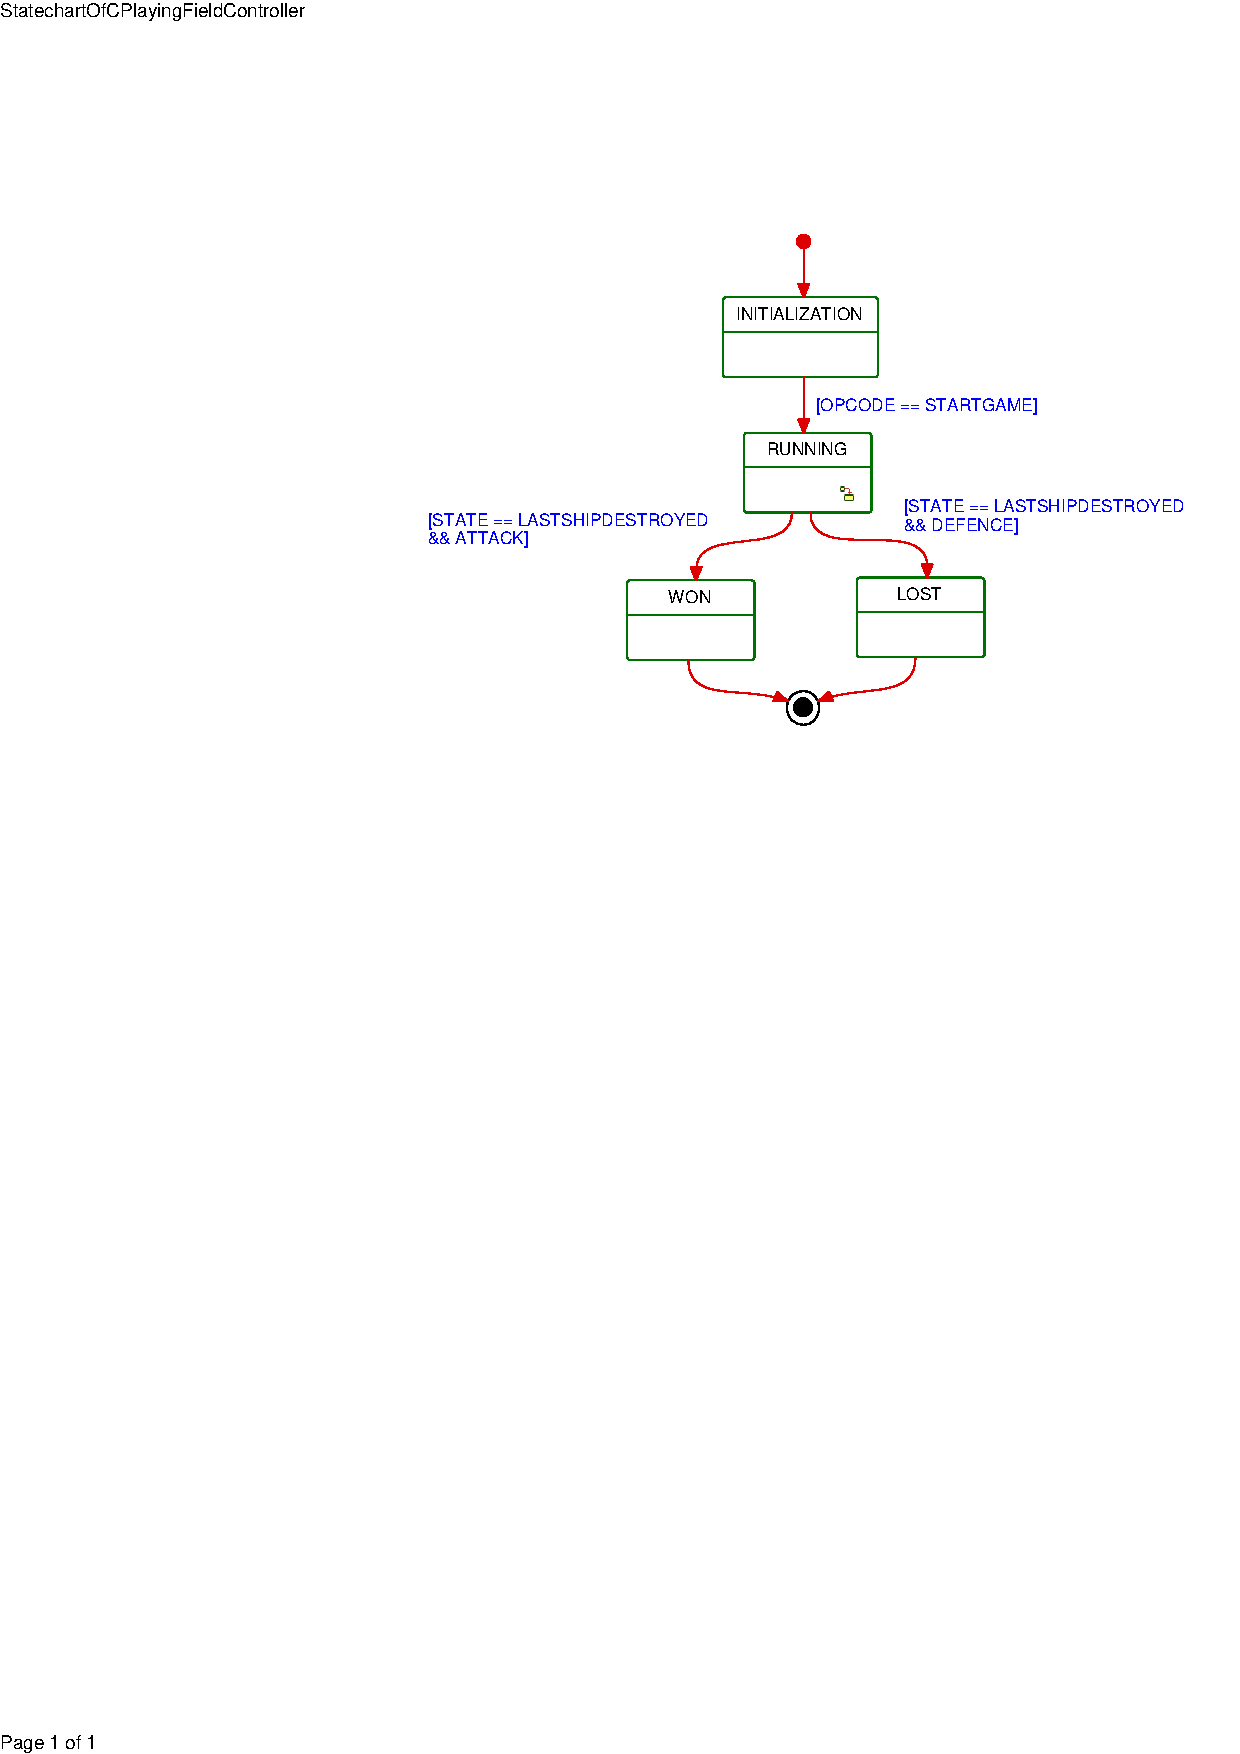
\includegraphics[trim=105mm 155mm 5mm 42mm,clip,width=0.5\textwidth]{images/SMController.pdf}
  \caption{Zustandsübergänge des Clients}
  \label{fig:Clientstates}
\end{figure}


\begin{figure}[H]
  \centering
  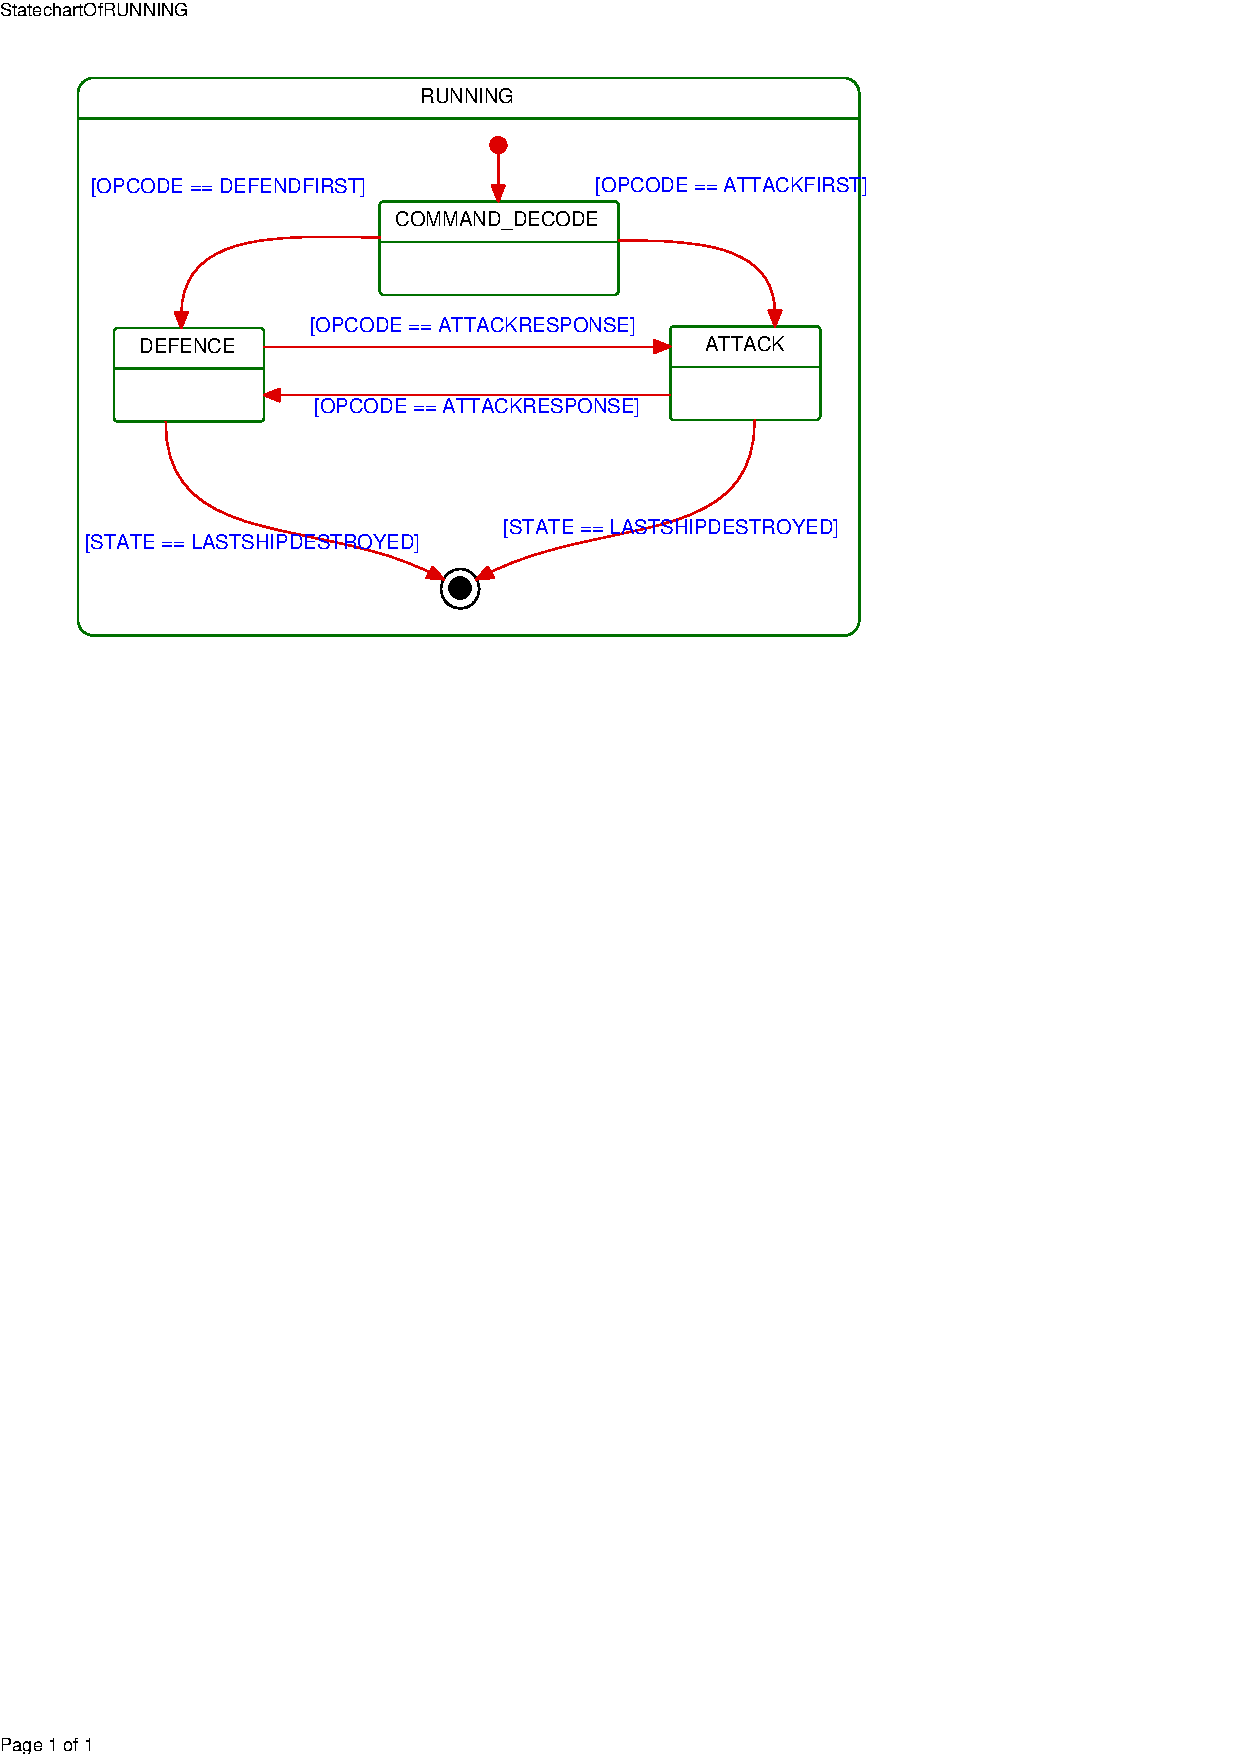
\includegraphics[trim=10mm 185mm 60mm 10mm,clip,width=0.5\textwidth]{images/SubSMRUNNING.pdf}
  \caption{Interne Zustandsübergänge während des laufenden Spiels}
  \label{fig:SubClientstates}
\end{figure}


\begin{figure}[H]
  \centering
  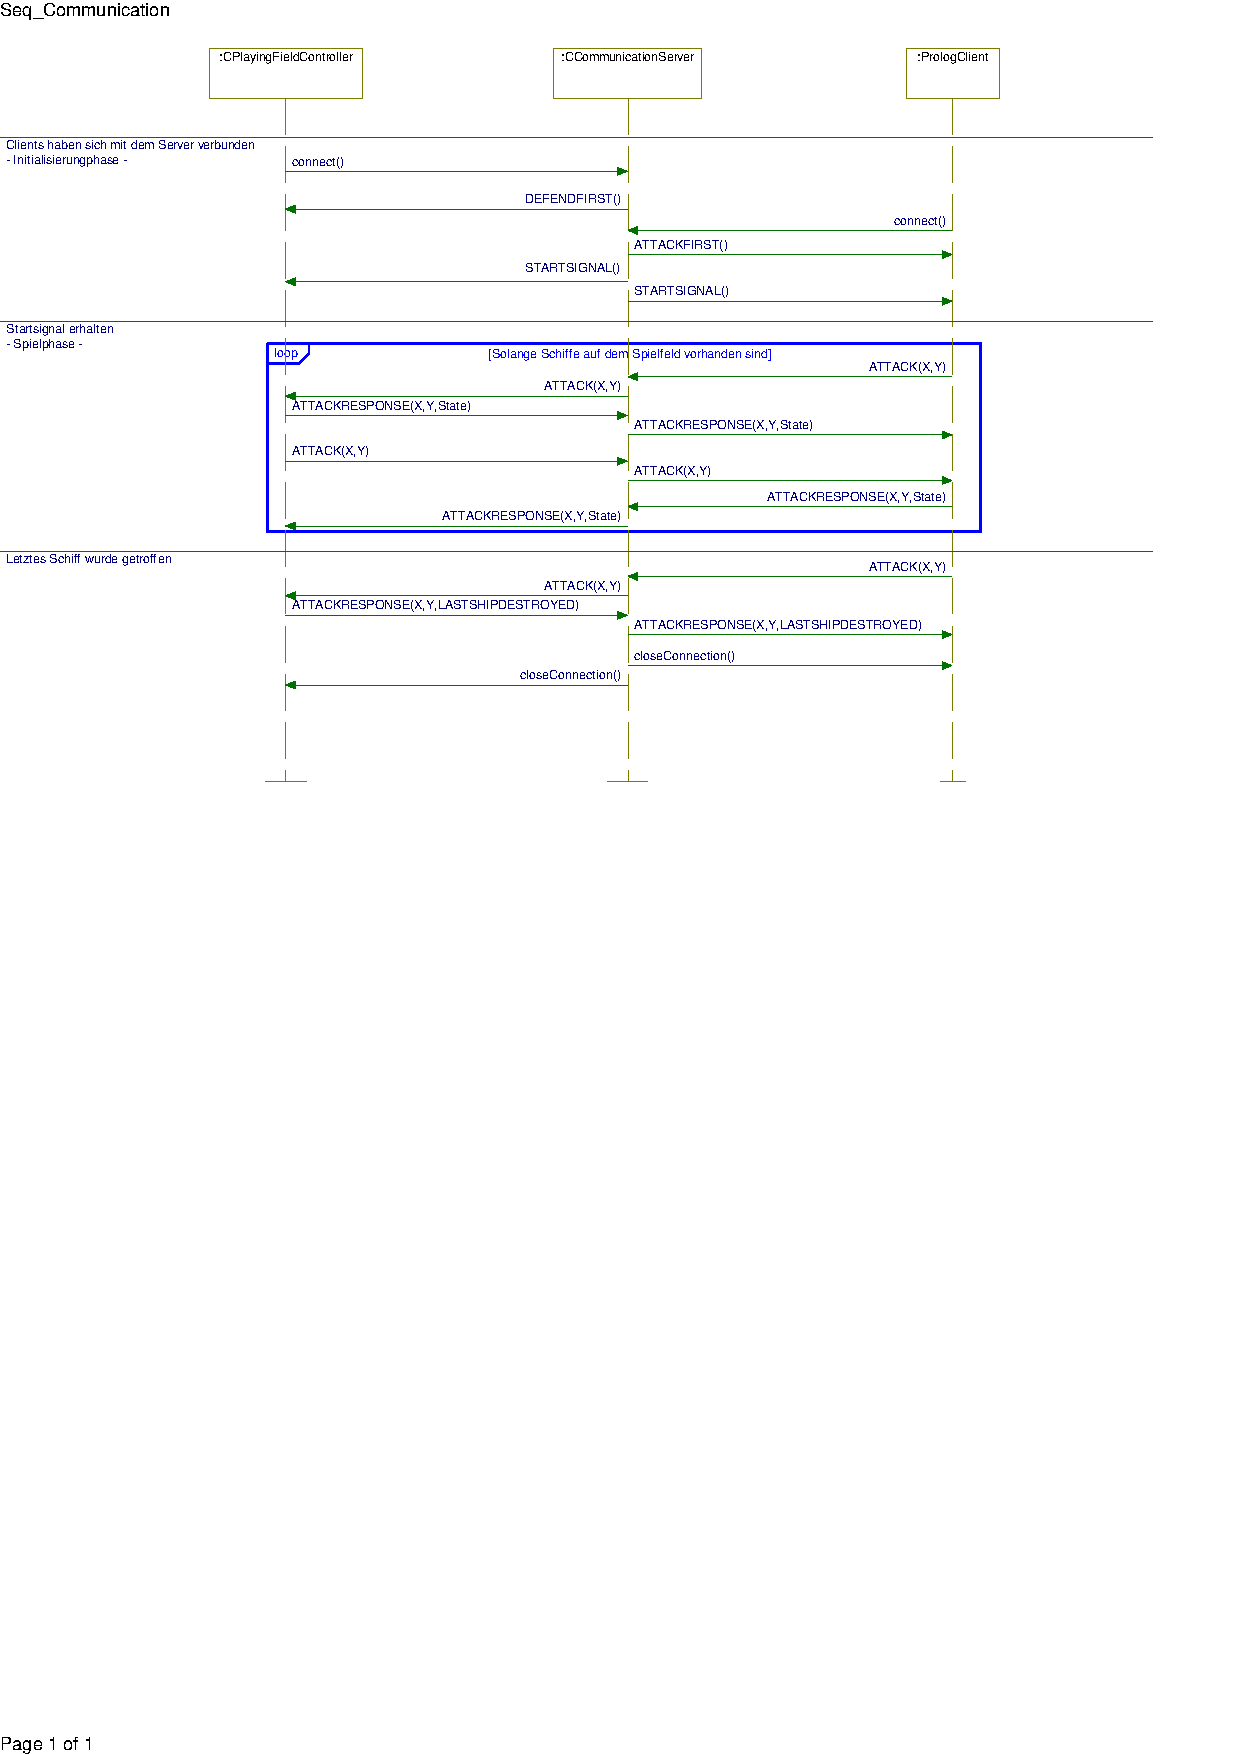
\includegraphics[trim=0mm 160mm 25mm 5mm,clip,width=0.9\textwidth]{images/SeqCommunication.pdf}
  \caption{Sequenzdiagramm der Kommunikation}
  \label{fig:Kommunikationssequenz}
\end{figure}

